%  A simple AAU report template.
%  2013-03-06 v. 1.0.0
%  Copyright 2010-2013 by Jesper Kjær Nielsen <jkn@es.aau.dk>
%
%  This is free software: you can redistribute it and/or modify
%  it under the terms of the GNU General Public License as published by
%  the Free Software Foundation, either version 3 of the License, or
%  (at your option) any later version.
%
%  This is distributed in the hope that it will be useful,
%  but WITHOUT ANY WARRANTY; without even the implied warranty of
%  MERCHANTABILITY or FITNESS FOR A PARTICULAR PURPOSE.  See the
%  GNU General Public License for more details.
%
%  You can find the GNU General Public License at <http://www.gnu.org/licenses/>.
%
%  A simple AAU report template.
%  2013-03-06 v. 1.0.0
%  Copyright 2010-2013 by Jesper Kjær Nielsen <jkn@es.aau.dk>
%
%  This is free software: you can redistribute it and/or modify
%  it under the terms of the GNU General Public License as published by
%  the Free Software Foundation, either version 3 of the License, or
%  (at your option) any later version.
%
%  This is distributed in the hope that it will be useful,
%  but WITHOUT ANY WARRANTY; without even the implied warranty of
%  MERCHANTABILITY or FITNESS FOR A PARTICULAR PURPOSE.  See the
%  GNU General Public License for more details.
%
%  You can find the GNU General Public License at <http://www.gnu.org/licenses/>.
%
\documentclass[11pt,twoside,a4paper,openright]{report}

%%%%%%%%%%%%%%%%%%%%%%%%%%%%%%%%%%%%%%%%%%%%%%%%
% Language, Encoding and Fonts
% http://en.wikibooks.org/wiki/LaTeX/Internationalization
%%%%%%%%%%%%%%%%%%%%%%%%%%%%%%%%%%%%%%%%%%%%%%%%
% Select encoding of your inputs. Depends on
% your operating system and its default input
% encoding. Typically, you should use
%   Linux  : utf8 (most modern Linux distributions)
%            latin1 
%   Windows: ansinew
%            latin1 (works in most cases)
%   Mac    : applemac
% Notice that you can manually change the input
% encoding of your files by selecting "save as"
% an select the desired input encoding. 
\usepackage[utf8]{inputenc}
% Make latex understand and use the typographic
% rules of the language used in the document.
\usepackage[danish,english]{babel}
% Use the vector font Latin Modern which is going
% to be the default font in latex in the future.
\usepackage{lmodern}
% Choose the font encoding
\usepackage[T1]{fontenc}
\usepackage{float}
%%%%%%%%%%%%%%%%%%%%%%%%%%%%%%%%%%%%%%%%%%%%%%%%
% Graphics and Tables
% http://en.wikibooks.org/wiki/LaTeX/Importing_Graphics
% http://en.wikibooks.org/wiki/LaTeX/Tables
% http://en.wikibooks.org/wiki/LaTeX/Colors
%%%%%%%%%%%%%%%%%%%%%%%%%%%%%%%%%%%%%%%%%%%%%%%%
% load a colour package
\usepackage{xcolor}
\definecolor{aaublue}{RGB}{33,26,82}% dark blue
% The standard graphics inclusion package
\usepackage{graphicx}
% Set up how figure and table captions are displayed
\usepackage{caption}
\captionsetup{%
  font=footnotesize,% set font size to footnotesize
  labelfont=bf % bold label (e.g., Figure 3.2) font
}
% Make the standard latex tables look so much better
\usepackage{array,booktabs}
% Enable the use of frames around, e.g., theorems
% The framed package is used in the example environment
\usepackage{framed}

%%%%%%%%%%%%%%%%%%%%%%%%%%%%%%%%%%%%%%%%%%%%%%%%
% Mathematics
% http://en.wikibooks.org/wiki/LaTeX/Mathematics
%%%%%%%%%%%%%%%%%%%%%%%%%%%%%%%%%%%%%%%%%%%%%%%%
% Defines new environments such as equation,
% align and split 
\usepackage{amsmath}
% Adds new math symbols
\usepackage{amssymb}
% Use theorems in your document
% The ntheorem package is also used for the example environment
% When using thmmarks, amsmath must be an option as well. Otherwise \eqref doesn't work anymore.
\usepackage[framed,amsmath,thmmarks]{ntheorem}

%%%%%%%%%%%%%%%%%%%%%%%%%%%%%%%%%%%%%%%%%%%%%%%%
% Page Layout
% http://en.wikibooks.org/wiki/LaTeX/Page_Layout
%%%%%%%%%%%%%%%%%%%%%%%%%%%%%%%%%%%%%%%%%%%%%%%%
% Change margins, papersize, etc of the document
\usepackage[
  left=28mm,% left margin on an odd page
  right=41mm,% right margin on an odd page
  ]{geometry}
% Modify how \chapter, \section, etc. look
% The titlesec package is very configureable
\usepackage{titlesec}
\titleformat*{\section}{\normalfont\Large\bfseries\color{aaublue}}
\titleformat*{\subsection}{\normalfont\large\bfseries\color{aaublue}}
\titleformat*{\subsubsection}{\normalfont\normalsize\bfseries\color{aaublue}}
%\titleformat*{\paragraph}{\normalfont\normalsize\bfseries\color{aaublue}}
%\titleformat*{\subparagraph}{\normalfont\normalsize\bfseries\color{aaublue}}

% Change the headers and footers
\usepackage{fancyhdr}
\pagestyle{fancy}
\fancyhf{} %delete everything
\renewcommand{\headrulewidth}{0pt} %remove the horizontal line in the header
\fancyhead[RE]{\color{aaublue}\small\nouppercase\leftmark} %even page - chapter title
\fancyhead[LO]{\color{aaublue}\small\nouppercase\rightmark} %uneven page - section title
\fancyhead[LE,RO]{\thepage} %page number on all pages
% Do not stretch the content of a page. Instead,
% insert white space at the bottom of the page
\raggedbottom
% Enable arithmetics with length. Useful when
% typesetting the layout.
\usepackage{calc}

%%%%%%%%%%%%%%%%%%%%%%%%%%%%%%%%%%%%%%%%%%%%%%%%
% Bibliography
% http://en.wikibooks.org/wiki/LaTeX/Bibliography_Management
%%%%%%%%%%%%%%%%%%%%%%%%%%%%%%%%%%%%%%%%%%%%%%%%
% Add the \citep{key} command which display a
% reference as [author, year]
\usepackage[square]{natbib}
% Appearance of the bibliography
\bibliographystyle{apalike}

%%%%%%%%%%%%%%%%%%%%%%%%%%%%%%%%%%%%%%%%%%%%%%%%
% Misc
%%%%%%%%%%%%%%%%%%%%%%%%%%%%%%%%%%%%%%%%%%%%%%%%
% Add bibliography and index to the table of
% contents
\usepackage[nottoc]{tocbibind}
% Add the command \pageref{LastPage} which refers to the
% page number of the last page
\usepackage[
%  disable, %turn off todonotes
  colorinlistoftodos, %enable a coloured square in the list of todos
  textwidth=\marginparwidth, %set the width of the todonotes
  textsize=scriptsize, %size of the text in the todonotes
  ]{todonotes}
% added by KK (ShareLaTeX team)
\usepackage{lastpage}

%%%%%%%%%%%%%%%%%%%%%%%%%%%%%%%%%%%%%%%%%%%%%%%%
% Hyperlinks
% http://en.wikibooks.org/wiki/LaTeX/Hyperlinks
%%%%%%%%%%%%%%%%%%%%%%%%%%%%%%%%%%%%%%%%%%%%%%%%
% Enable hyperlinks and insert info into the pdf
% file. Hypperref should be loaded as one of the 
% last packages
\usepackage{hyperref}
\hypersetup{%
	pdfpagelabels=true,%
	plainpages=false,%
	pdfauthor={Author(s)},%
	pdftitle={Title},%
	pdfsubject={Subject},%
	bookmarksnumbered=true,%
	colorlinks,%
	citecolor=aaublue,%
	filecolor=aaublue,%
	linkcolor=aaublue,% you should probably change this to black before printing
	urlcolor=aaublue,%
	pdfstartview=FitH%
}

% package inclusion and set up of the document
% see, e.g., http://en.wikibooks.org/wiki/LaTeX/Formatting#Hyphenation
% for more information on word hyphenation
\hyphenation{ex-am-ple hy-phen-a-tion short}
\hyphenation{long la-tex}
% 
%  A simple AAU report template.
%  2013-03-06 v. 1.0.0
%  Copyright 2010-2013 by Jesper Kjær Nielsen <jkn@es.aau.dk>
%
%  This is free software: you can redistribute it and/or modify
%  it under the terms of the GNU General Public License as published by
%  the Free Software Foundation, either version 3 of the License, or
%  (at your option) any later version.
%
%  This is distributed in the hope that it will be useful,
%  but WITHOUT ANY WARRANTY; without even the implied warranty of
%  MERCHANTABILITY or FITNESS FOR A PARTICULAR PURPOSE.  See the
%  GNU General Public License for more details.
%
%  You can find the GNU General Public License at <http://www.gnu.org/licenses/>.
%
%
%
% see, e.g., http://en.wikibooks.org/wiki/LaTeX/Customizing_LaTeX#New_commands
% for more information on how to create macros

%%%%%%%%%%%%%%%%%%%%%%%%%%%%%%%%%%%%%%%%%%%%%%%%
% Macros for the titlepage
%%%%%%%%%%%%%%%%%%%%%%%%%%%%%%%%%%%%%%%%%%%%%%%%
%Creates the aau titlepage
\newcommand{\aautitlepage}[3]{%
  {
    %set up various length
    \ifx\titlepageleftcolumnwidth\undefined
      \newlength{\titlepageleftcolumnwidth}
      \newlength{\titlepagerightcolumnwidth}
    \fi
    \setlength{\titlepageleftcolumnwidth}{0.5\textwidth-\tabcolsep}
    \setlength{\titlepagerightcolumnwidth}{\textwidth-2\tabcolsep-\titlepageleftcolumnwidth}
    %create title page
    \thispagestyle{empty}
    \noindent%
    \begin{tabular}{@{}ll@{}}
      \parbox{\titlepageleftcolumnwidth}{
        \iflanguage{danish}{%
          
\includegraphics[width=\titlepageleftcolumnwidth]{figures/aau_logo_da}
        }{%
          
\includegraphics[width=\titlepageleftcolumnwidth]{figures/aau_logo_en}
        }
      } &
      \parbox{\titlepagerightcolumnwidth}{\raggedleft\sf\small
        #2
      }\bigskip\\
       #1 &
      \parbox[t]{\titlepagerightcolumnwidth}{%
      \textbf{Abstract:}\bigskip\par
        \fbox{\parbox{\titlepagerightcolumnwidth-2\fboxsep-2\fboxrule}{%
          #3
        }}
      }\\
    \end{tabular}
    \vfill
    \iflanguage{danish}{%
      \noindent{\footnotesize\emph{Rapportens indhold er frit tilgængeligt, men offentliggørelse (med kildeangivelse) må kun ske efter aftale med forfatterne.}}
    }{%
      \noindent{\footnotesize\emph{The content of this report is freely available, but publication (with reference) may only be pursued due to agreement with the author.}}
    }
    \clearpage
  }
}

%Create english project info
\newcommand{\englishprojectinfo}[8]{%
  \parbox[t]{\titlepageleftcolumnwidth}{
    \textbf{Title:}\\ #1\bigskip\par
    \textbf{Theme:}\\ #2\bigskip\par
    \textbf{Project Period:}\\ #3\bigskip\par
    \textbf{Project Group:}\\ #4\bigskip\par
    \textbf{Participant(s):}\\ #5\bigskip\par
    \textbf{Supervisor(s):}\\ #6\bigskip\par
    \textbf{Copies:} #7\bigskip\par
    \textbf{Page Numbers:} \pageref{LastPage}\bigskip\par
    \textbf{Date of Completion:}\\ #8
  }
}

%Create danish project info
\newcommand{\danishprojectinfo}[8]{%
  \parbox[t]{\titlepageleftcolumnwidth}{
    \textbf{Titel:}\\ #1\bigskip\par
    \textbf{Tema:}\\ #2\bigskip\par
    \textbf{Projektperiode:}\\ #3\bigskip\par
    \textbf{Projektgruppe:}\\ #4\bigskip\par
    \textbf{Deltager(e):}\\ #5\bigskip\par
    \textbf{Vejleder(e):}\\ #6\bigskip\par
    \textbf{Oplagstal:} #7\bigskip\par
    \textbf{Sidetal:} \pageref{LastPage}\bigskip\par
    \textbf{Afleveringsdato:}\\ #8
  }
}

%%%%%%%%%%%%%%%%%%%%%%%%%%%%%%%%%%%%%%%%%%%%%%%%
% An example environment
%%%%%%%%%%%%%%%%%%%%%%%%%%%%%%%%%%%%%%%%%%%%%%%%
\theoremheaderfont{\normalfont\bfseries}
\theorembodyfont{\normalfont}
\theoremstyle{break}
\def\theoremframecommand{{\color{aaublue!50}\vrule width 5pt \hspace{5pt}}}
\newshadedtheorem{exa}{Example}[chapter]
\newenvironment{example}[1]{%
		\begin{exa}[#1]
}{%
		\end{exa}
}
% my new macros

\begin{document}
%frontmatter
\pagestyle{empty} %disable headers and footers
\pagenumbering{roman} %use roman page numbering in the frontmatter
%  A simple AAU report template.
%  2013-03-06 v. 1.0.0
%  Copyright 2010-2013 by Jesper Kjær Nielsen <jkn@es.aau.dk>
%
%  This is free software: you can redistribute it and/or modify
%  it under the terms of the GNU General Public License as published by
%  the Free Software Foundation, either version 3 of the License, or
%  (at your option) any later version.
%
%  This is distributed in the hope that it will be useful,
%  but WITHOUT ANY WARRANTY; without even the implied warranty of
%  MERCHANTABILITY or FITNESS FOR A PARTICULAR PURPOSE.  See the
%  GNU General Public License for more details.
%
%  You can find the GNU General Public License at <http://www.gnu.org/licenses/>.
%
\pdfbookmark[0]{Front page}{label:frontpage}%
\begin{titlepage}
  \addtolength{\hoffset}{0.5\evensidemargin-0.5\oddsidemargin} %set equal margins on the frontpage - remove this line if you want default margins
  \noindent%
  \begin{tabular}{@{}p{\textwidth}@{}}
    \toprule[2pt]
    \midrule
    \vspace{0.2cm}
    \begin{center}
    \Huge{\textbf{
      Linearisation of multiple RF-power amplifiers with the presentence of antenna crosstalk % insert your title here
    }}
    \end{center}
    \begin{center}
      \Large{
         Master thesis % insert your subtitle here
      }
    \end{center}
    \vspace{0.2cm}\\
    \midrule
    \toprule[2pt]
  \end{tabular}
  \vspace{4 cm}
  \begin{center}
    {\large
      Author%Insert document type (e.g., Project Report)
    }\\
    \vspace{0.2cm}
    {\Large
      Karsten Schou Nielsen%Insert your group name or real names here
    }
  \end{center}
  \vfill
  \begin{center}
  Aalborg University\\
  Department of Antennas, Propagation and Millimetre-Wave Systems (APMS)\\
  Selma Lagerløfs Vej 312\\
  DK-9220 Aalborg
  \end{center}
\end{titlepage}
\clearpage

\thispagestyle{empty}
{\small
\strut\vfill % push the content to the bottom of the page
\noindent Copyright \copyright{} Aalborg University 2019\par
\vspace{0.2cm}
\noindent 
}
\clearpage


\pdfbookmark[0]{English title page}{label:titlepage_en}
\aautitlepage{%
  \englishprojectinfo{
    Deployable Quadrifilar Helical Antenna for space application %title
  }{%
    Scientific Theme %theme
  }{%
    Fall Semester 2018 %project period
  }{%
    XXX % project group
  }{%
    %list of group members
	Karsten Schou Nielsen
  }{%
    %list of supervisors
	Ming Shen
  }{%
    1 % number of printed copies
  }{%
    \today % date of completion
  }%
}{%department and address
  \textbf{Department of Electronic Systems}\\
  Fredrik Bajers Vej 7\\
  DK-9220 Aalborg Ø\\
  \href{http://es.aau.dk}{http://es.aau.dk}
}{% the abstract
  Here is the abstract
}

\cleardoublepage
{\selectlanguage{danish}
\pdfbookmark[0]{Danish title page}{label:titlepage_da}
\aautitlepage{%
  \danishprojectinfo{
    Deployable Quadrifilar Helical Antenna for space application %title
  }{%
    Semestertema %theme
  }{%
    Efterårssemestret 2018 %project period
  }{%
    XXX % project group
  }{%
    %list of group members
    Karsten Schou Nielsen\\ 

  }{%
    %list of supervisors
    Ming Shen\\
  }{%
    1 % number of printed copies
  }{%
    \today % date of completion
  }%
}{%department and address
  \textbf{Institut for Elektroniske Systemer}\\
  Fredrik Bajers Vej 7\\
  DK-9220 Aalborg Ø\\
  \href{http://es.aau.dk}{http://es.aau.dk}
}{% the abstract
  Her er resuméet
}}

\cleardoublepage
\pdfbookmark[0]{Contents}{label:contents}
\pagestyle{fancy} %enable headers and footers again
\tableofcontents
\listoftodos
\chapter*{Preface\markboth{Preface}{Preface}}\label{ch:preface}
\addcontentsline{toc}{chapter}{Preface}
This thesis project has been carried out within the Antennas, Propagation and Millimetre-Wave Systems (AMPS) at Aalborg University Denmark under supervision of associate professor Ming Shen. I am thankful for this valuable experience at the university and
by the new knowledge I have acquired, as well as by the global atmosphere at AMPS. I hope that this work will be helpful for others in the same area in the future. 
    

\vspace{\baselineskip}\hfill Aalborg University, \today
\vfill\noindent
\begin{center}
\begin{minipage}[b]{0.45\textwidth}
 \centering
 \rule{\textwidth}{0.5pt}\\
  Karsten Schou Nielsen \\
 {\footnotesize <ksni12@student.aau.dk>}
\end{minipage}
\end{center}
%\hfill
%\begin{minipage}[b]{0.45\textwidth}
% \centering
% \rule{\textwidth}{0.5pt}\\
%  Author 2\\
% {\footnotesize <username2@XX.aau.dk>}
%\end{minipage}
%\vspace{3\baselineskip}
%\begin{center}
%\begin{minipage}[b]{0.45\textwidth}
% \centering
% \rule{\textwidth}{0.5pt}
%  Author 3\\
% {\footnotesize <username3@XX.aau.dk>}
%\end{minipage}
%\end{center}

\cleardoublepage
%mainmatter
\pagenumbering{arabic} %use arabic page numbering in the mainmatter
\chapter{Introduction}\label{ch:introduction}

This master thesis is aiming at the linearization of Power amplifiers with the presence of cross talk in antenna arrays. The tasks include  - the characterization of the cross talk and its impact on the system linearity
- digital pre-distrotion of PAs under effects of antenna cross talks. The project is motivated by the quickly growing need from the mobile communication industry, where highly integrated beam-steerable arrays consisting of a big number of power amplifiers and antenna elements are considered as the solution for higher data rates desired in emerging applications such as self-driving cars, remote e-health etc. There will be use DPD techniques that can capture the total nonlinearity of the whole array including the PAs and antenna elements. The special focus is to reduce the system complexity, while maintaining the linearisation performance. 

This project will be conducted in a way combining mainly measurements together with computaion in MATLAB



\chapter{linkbudget}\label{ch:linkbudget}

Typically in satellite communication a LOS component exist. Therefore the only obstacle between the satellite and user is the atmosphere and therefore the loss can be modelled as free space, with a limited variation due to weather conditions. ADS-B signal is sent through a linear polarized monopol with power varying from 75 W to 500 W depending of the airplane and speed \citep{FlyingLab}. The height of a low orbit satellite is between 600 km to 800 km. To calculate the power loss Friis Transmission Equation is used. It is assumed that the SNIR is minimum 9dB \citep{itu} 

\begin{equation}
\frac{P_r}{P_t} = (\frac{\lambda}{4\pi R})^2 G_t G_r|\vec{Pr}\cdot \vec{Pt}|^2
\end{equation}

\begin{equation}
\lambda = \frac{c}{f}
\end{equation}
Where $c = 3e8$ is speed of light in vaccum and $ f$ is the frequency in Hz. $|\vec{Pr}\cdot \vec{Pt}|^2$ denotes polarization mishmash. When solving for $f = 137MHz$ $R=800km$  $G_t = 0 dB$ and a polarization loss at 0, the free-space loss becomes 133.2dB.


\begin{center}
  \begin{tabular}{ l  l  l  l  l}
    \hline
   \textit{Item} & \textit{Link parameter} & \textit{Value} & \textit{Unit} & \textit{Computation} \\ \hline
    1 & Frequency	& 1090 & MHz & \\ \hline
    2 & Transmit power (75W) & 18.8 & dB & \\ \hline
    3 & Transmit antenna gain & 3 & dBi & \\ \hline
    4 & Athmospheric absorbtion (clean air) & 0.1 & dB & \\ \hline
    5 & Free-space loss & 151.3 & dB & \\ \hline
    6 & Polarisation loss & 3 & dB & \\ \hline
    7 & Received carrier power & -135.6 & dB & 2+3-4-5\\ \hline
    8 & Bandwith (4.6MHz) & 66.6 & dB Hz & \\ \hline 
    9 & System noise temperature (373K) & 25.7 & dBK& \\ \hline 
    10 & Boltzmann's constant & -228.6 & dBW/Hz/K& \\ \hline 
    11 & Noise power & -136.6 & dBW& 8+9+10\\ \hline 
    12 & Carrier to noise ratio & 7.0 & db & 7-11\\ \hline 
    13 & C/(N+I) & 9 & db & Requirement\\ \hline
    14 & Receive antenna gain & 2 & db & 13-12\\ \hline
  \end{tabular}
\end{center}


\chapter{Antennas}\label{ch:antennas}

With the requirements calculated in chapter \ref{ch:linkbudget}, it is now possible to design an antenna to overcome these requirements.  

\section{Dipole antennas}


\section{Reflector Antennas}

Reflector antennas are used places where a high gain and directivity is needed. The reflector antenna do also have a wide bandwith, which all together has made them poplar for deep space communication \citep{Imbriale2012}. Although reflector antennas can be made in different types, shapes and configurations, they all essentially consist of a passive reflecting surface illuminated by a smaller primary feed. The basic analysis is done using trigonometry which provides satisfactory result because the diameter of the reflecting surface often is ten times the wavelength. In figure \ref{fig:reflector_types} four main configurations is depicted. (a) is the on-focus parabolic reflector where the feed for the parabolic is placed F distance apart called the focal point. This would leave an area where the feed is placed, where there will be a gap in the coverage. This is omitted in (b) which is the off-axis reflector. This types has no gap in coverage and therefore is often used as radar. The (c) Cassegrain reflector and (d) Gregorian reflector uses both a feed in the middle of the reflector which then uses a second reflector at the focal point to reflect the energy back to the large reflector. Because of the large dimensions a reflector antenna are not suited for low frequencies < 2GHz. Using the equations \ref{eq:para1} to \ref{eq:para4} a design has been made for $f = 10GHz$, $\lambda = 30mm$, $D = 10\lambda = 300mm$, $\theta = 60^{\circ}$. This should give a gain at 30dBi. The design has been simulated in CST studio in figure \ref{fig:para_sim1} and \ref{fig:para_sim2}. The feeding antenna used is a dipole which is an omnidirectional antenna, this causes a loss in efficiency. An ideal reflector should be uniformly illuminated and all power should
be focused on the reflecting surface. The portion of the feed power that does not reach the reflector is referred to
as spillover loss while the ability to uniformly feed the parabola is referred to as illumination efficiency. Since
primary feeds have a tapered radiation pattern, a compromise between spillover losses and illumination
efficiency must be considered to maximize the aperture gain. In the simulation a gain at $G=15dB$ was obtained, this could be optimized using an horn-antenna. 

\begin{figure}[H]
\centering 
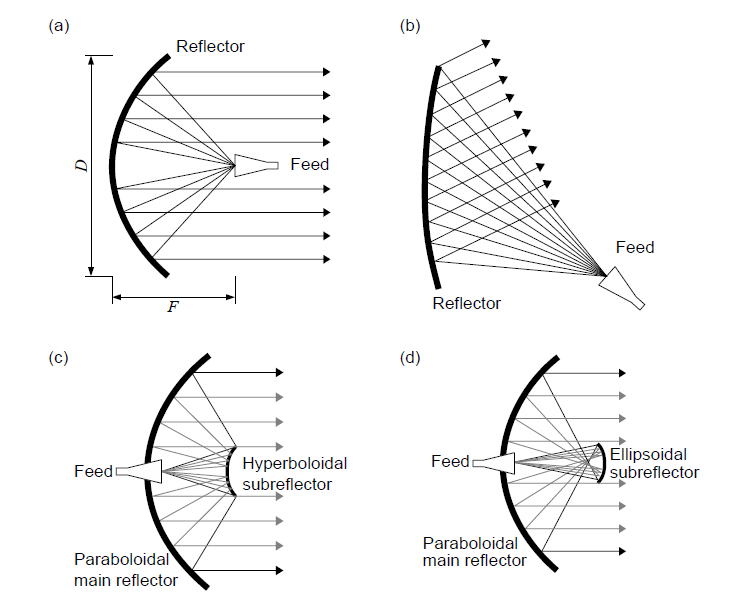
\includegraphics[scale = 0.7]{figures/antennas/reflector/types}
\caption{Reflector antenna configurations: (a) on-focus parabolic reflector; (b) off-axis reflector; (c) Cassegrain reflector; (d) Gregorian reflector \citep{Imbriale2012}}
\label{fig:reflector_types}
\end{figure}

Equation for parabola

\begin{equation}
y=a x^2 , a = \frac{1}{4F}
\end{equation}
\label{eq:para1}

Focal length
\begin{equation}
F=D\frac{1}{4tan(\theta/4)}
\end{equation}
\label{eq:para2}

Length of parabolic segment
\begin{equation}
L=\frac{ln(\sqrt{a^2 D^2 +1}+a D)}{4a}+\frac{D\sqrt{a^2 D^2 +1}}{4}
\end{equation}
\label{eq:para3}

Gain for parabolic reflector

\begin{equation}
G=\eta \frac{4\pi A}{\lambda^2}, A = \frac{\pi D^2}{4}
\end{equation}
\label{eq:para4}

\begin{figure}[H]
\centering 
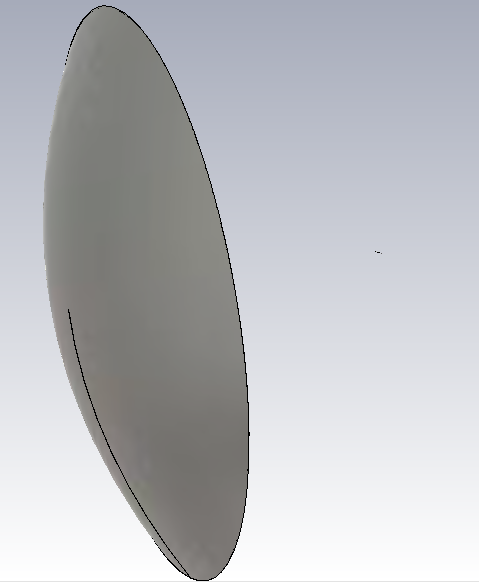
\includegraphics[scale = 0.5]{figures/antennas/reflector/parabola_cst}
\caption{Simulated reflector antenna in CST studio}
\label{fig:para_sim1}
\end{figure}

\begin{figure}[H]
\centering 
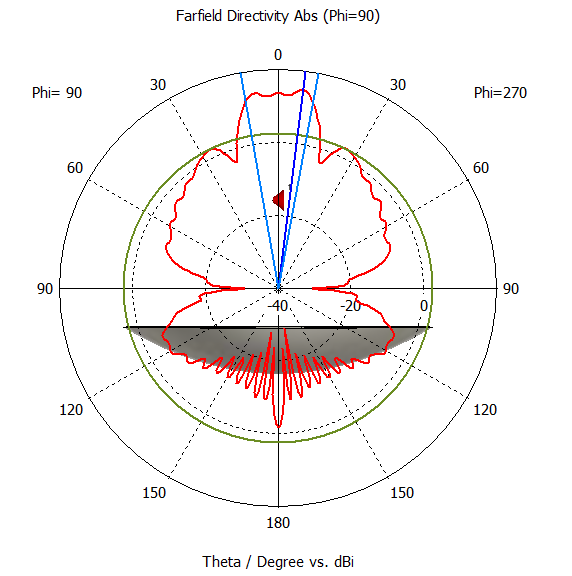
\includegraphics[scale = 0.5]{figures/antennas/reflector/parabola_cst_farfield}
\caption{Farfield of simulated reflector antenna in CST studio}
\label{fig:para_sim2}
\end{figure}



\section{Helical Antennas}
\subsection{Helical antenna with ground plane}

\begin{figure}[H]
\centering 
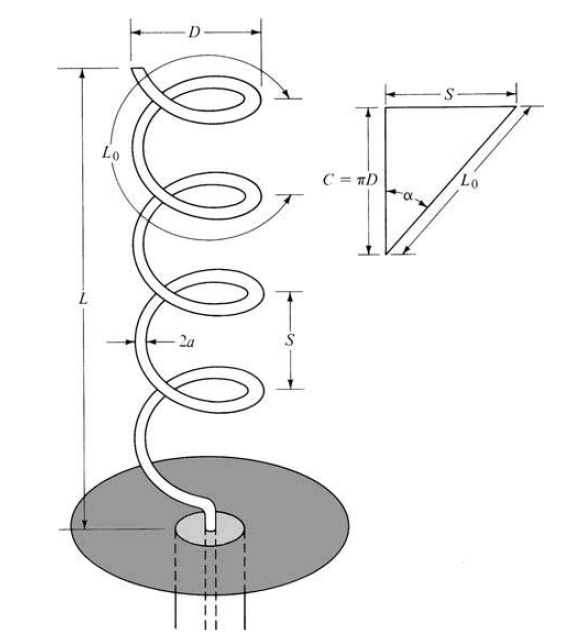
\includegraphics[scale = 0.5]{figures/antennas/helical/helical}
\caption{Helical antenna with ground plane \citep{Balanis2005}}
\label{fig:helical}
\end{figure}

\begin{figure}[H]
\centering 
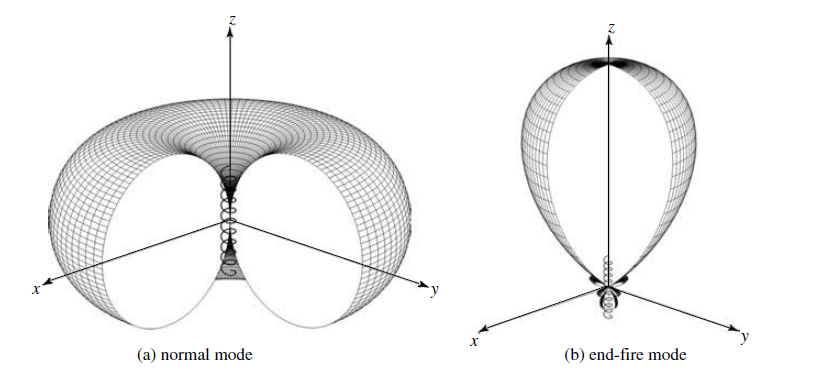
\includegraphics[scale = 0.5]{figures/antennas/helical/modes}
\caption{Farfield for (a) normal mode and (b)end-fire mode \citep{Balanis2005}}
\label{fig:helical_modes}
\end{figure}

A helical antenna is a wire wound in form of a screw and is depicted in figure \ref{fig:helical}. The helical antenna consist of N turns, diameter D and spacing between the turns S and circumference is $C = \pi D$w here the total length is $L = NS$. Normally the helical antenna has a circular ground plane with the diameter $G_d = \frac{3\lambda}{4}$. Another important parameter is the pitch angle $\alpha$ which is the angle formed by a line tangent to the helix wire and a plane perpendicular to the helix axis. The pitch angle is defined by   

\begin{equation}
\alpha = tan^{-1}(\frac{S}{\pi D}) = tan^{-1}(\frac{S}{C})
\end{equation} 

The radiation pattern of the antenna can be varied by controlling the size of its
geometrical properties compared to the wavelength. The input impedance is critically
dependent upon the pitch angle and the size of the conducting wire, especially near the
feed point, and it can be adjusted by controlling their values. The general polarization
of the antenna is elliptical. However circular and linear polarizations can be achieved
over different frequency ranges \citep{Balanis2005}. The helical antenna can operates typically in one of two modes which is
the normal (broadside) and the axial (end-fire) mode see figure \ref{fig:helical_modes}. In end-fire mode a circular polarization is archived if the D and S is large fractions of the wavelength. The design criteria is $\frac{3}{4} < C/\lambda < \frac{4}{3}$ where $C = \lambda$ is optimum. $S = \frac{\lambda}{4}$ this gives a pitch angle between $12^o \leq \alpha \leq 14^o $ and a ground plane at least $G_d = \frac{\lambda}{2}$. Formulas for radiation resistance Half Power Beam Width (HPBW) and reflection coefficient is given by equation \ref{eq:heli1} to \ref{eq:heli4}. The formulas has an accuracy about 20\% the formulas are therefore held up with a simulation at $f = 1GHz$.\\

Directivity
\begin{equation}
D =  15N\frac{C^2 S}{\lambda^3} = 12.7dB
\end{equation}  
\label{eq:heli1}

Half Power Beam Width
\begin{equation}
HPBW = \frac{52\lambda^{3/2} }{C\sqrt{NS}} = 46.5^o
\end{equation}  
\label{eq:heli2}

Impedance of antenna 
\begin{equation}
Z_l = 140\frac{C}{\lambda} = 140\Omega
\end{equation} 
\label{eq:heli3}
 
Reflection coefficient 
\begin{equation}
\Gamma = \frac{Z_l+Z_s}{Z_l-Z_s} = -3.2dB
\end{equation}  
\label{eq:heli4}

The simulation results are depicted in figure \ref{fig:helical_cst} to \ref{fig:helical_farfield}. It can be seen that the simulated results corresponds well with the formulas whit-in 20\% accuracy . 

\begin{figure}[H]
\centering 
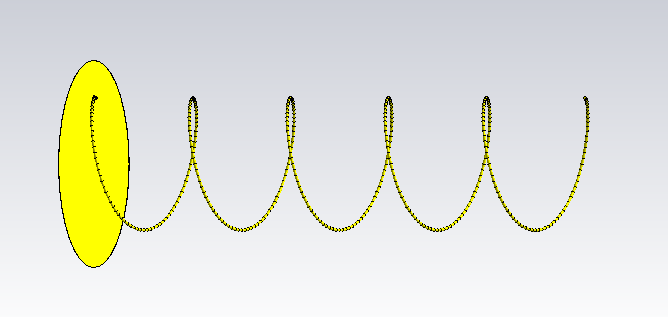
\includegraphics[scale = 0.5]{figures/antennas/helical/helical_cst}
\caption{Simulated helical antenna}
\label{fig:helical_cst}
\end{figure}

\begin{figure}[H]
\centering 
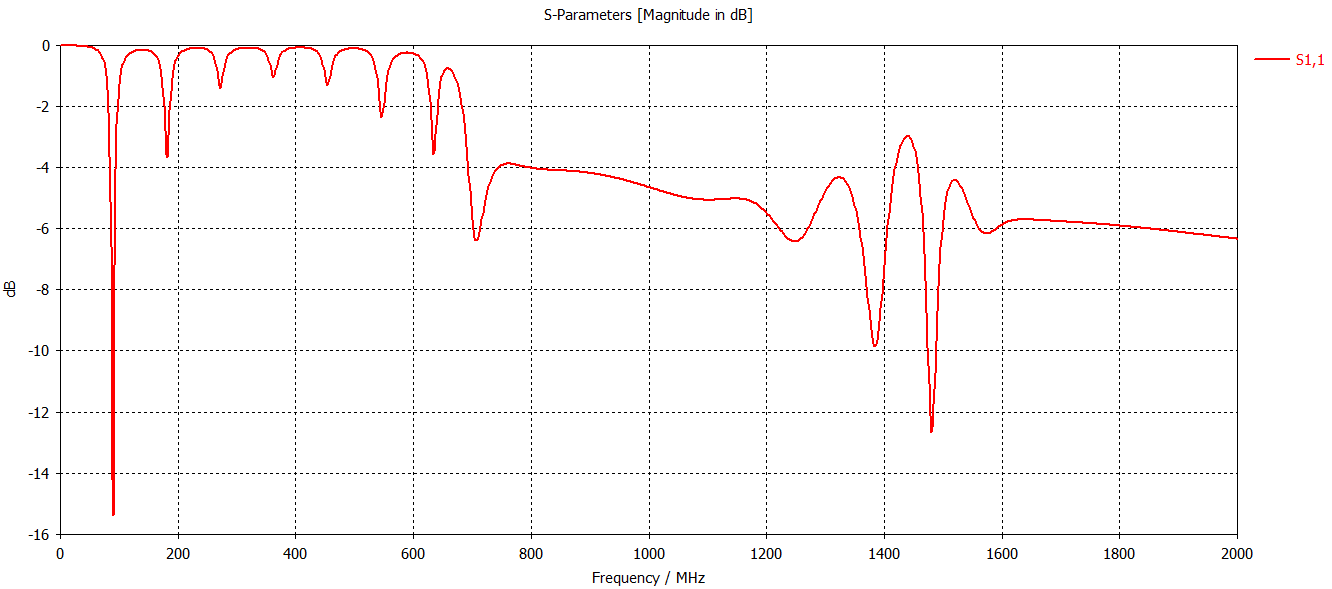
\includegraphics[scale = 0.5]{figures/antennas/helical/helical_cst_s11}
\caption{Reflection coefficient for simulated helical antenna}
\label{fig:helical_s11}
\end{figure}

\begin{figure}[H]
\centering 
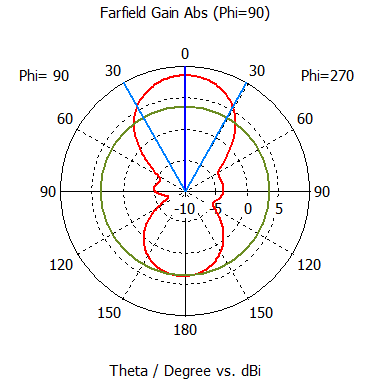
\includegraphics[scale = 0.5]{figures/antennas/helical/helical_cst_farfield}
\caption{Farfield for simulated helical antenna with a maximum directivity a 7.1dB and a HPBW at $58.8^o$}
\label{fig:helical_farfield}
\end{figure}

\subsection{Quadrifilar Helical Antenna}

\begin{figure}[H]
\centering 
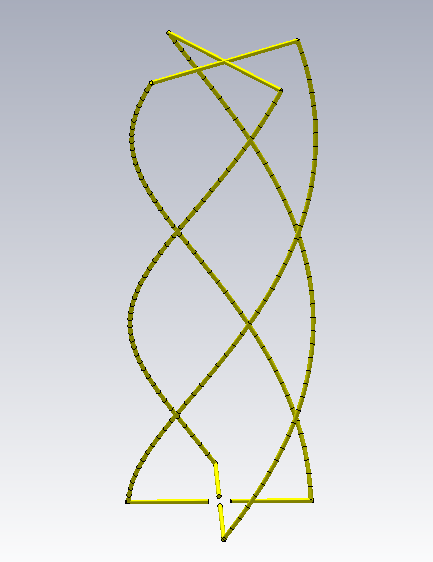
\includegraphics[scale = 0.7]{figures/antennas/qha/qha_6_1mhz}
\caption{QHA with $N=0.6$, $D=80mm$,$L=\frac{\lambda}{2}-D\cdot 0.75$, $f=1GHz$}
\label{fig:QHA1}
\end{figure}

The Quadrifilar Helical Antenna (QHA) (see figure \ref{fig:QHA1}) is an resonant antenna which is typically feed by two ports with a $90^\circ$ phase difference. The antenna has a circular polarization and the size is often smaller than a normal helical antenna. Typically the length of each arm is an integral multiple of the quarter-wavelength. The end of the helix
is open when the integer is odd, while short when the integer is
even \citep{Bai2014}. Despite the typically design the turn ratio, radius, length and feeding topology will affect the radiation pattern and polarization. Another important measure of all helical antennas is the pitch angle which is defined in equation \ref{eq:pitch}.

\begin{equation}
\alpha = tan^{-1}(\frac{S}{\pi D})
\end{equation}
\label{eq:pitch}

Where D is the diameter of the antenna, S is the spacing between the loops and futher N is the number of turns and L is the length of the antenna \citep{Balanis2005}.
\newline
\newline
An QHA has been build and simulated in CST studio. The dimensions are $D=80mm$,$L=\frac{\lambda}{2}-D\cdot 2$, $N=0.6$ at the frequency $f=122.5MHz$ and $\lambda = 2450mm$ with the wire diameter $Wd = 2mm$. The diameter is chosen so the antenna can be stowed in a 10x10x10cm box and the length is calculated so there is a half wavelength between the negative and positive side of a port. The feeding is done using two discrete ports as shoved in figure \ref{fig:QHA2}.  

\begin{figure}[H]
\centering 
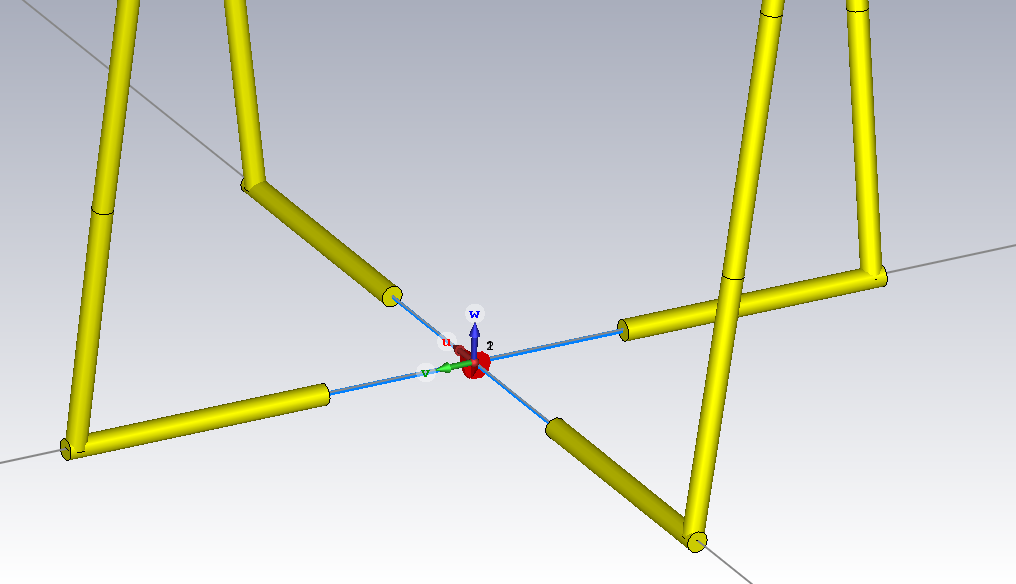
\includegraphics[scale = 0.4]{figures/antennas/qha/qha_6_feeding}
\caption{Feeding of the QHA for 122.5MHz using discrete ports}
\label{fig:QHA2}
\end{figure}
 
The QHA has been simulated and the results shows, that the antenna is matched to 131MHz even thou the S11 parameter at this frequency is only -2dB, see figure \ref{fig:QHA_S11}. The error is caused by the gap between the ports in the bottom and the extra length caused by the turn of N. It can be seen that the antenna also radiates at multiply of the match frequency and that the lowest return-loss is obtained at 4 times the frequency which gives 524MHz. The farfields for the frequencies 131,262 and 393MHz are shown in figure \ref{fig:QHA_ff_131}, \ref{fig:QHA_ff_262} and \ref{fig:QHA_ff_393}, where port 1 is fed with a positive phase at $90^\circ$. It is seen that the farfield not surprisingly changes with the frequency. The farfield suited best for tracking of ADS-B signals is the one in figure \ref{fig:QHA_ff_131}. \todo[inline,color=orange]{write someting about the earth curvature and why?}.      

\begin{figure}[H]
\centering 
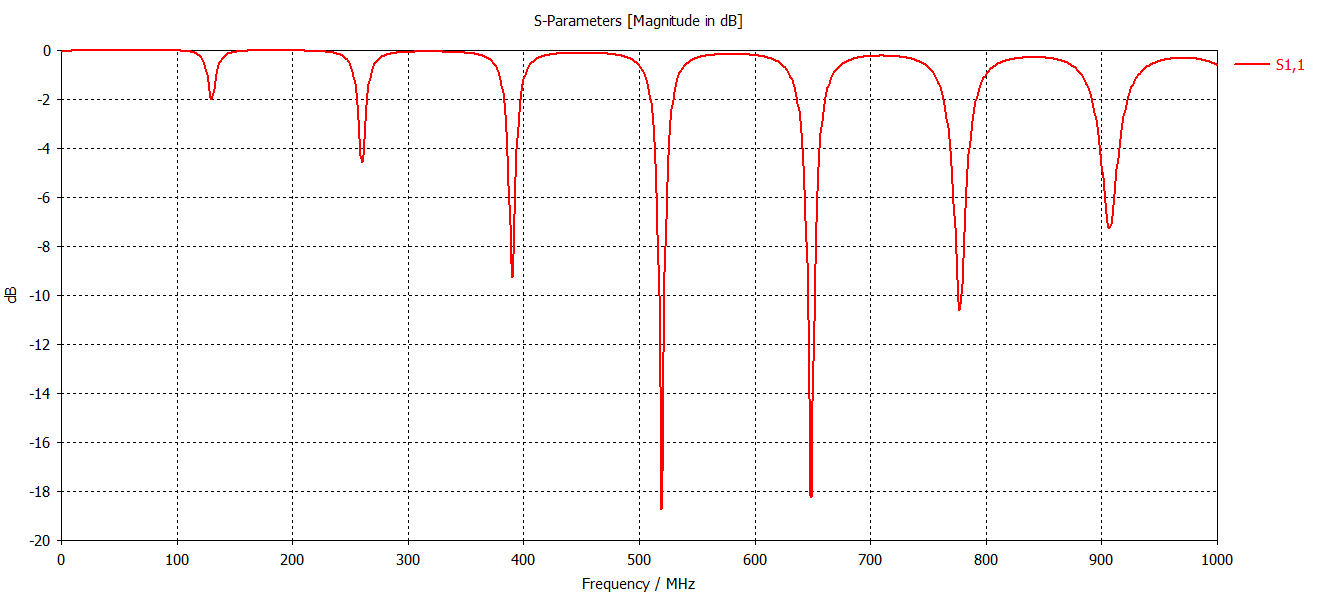
\includegraphics[scale = 0.5]{figures/antennas/qha/qha_6_S11}
\caption{S11 parameter of the QHA for 122.5MHz}
\label{fig:QHA_S11}
\end{figure}

\begin{figure}[H]
\centering 
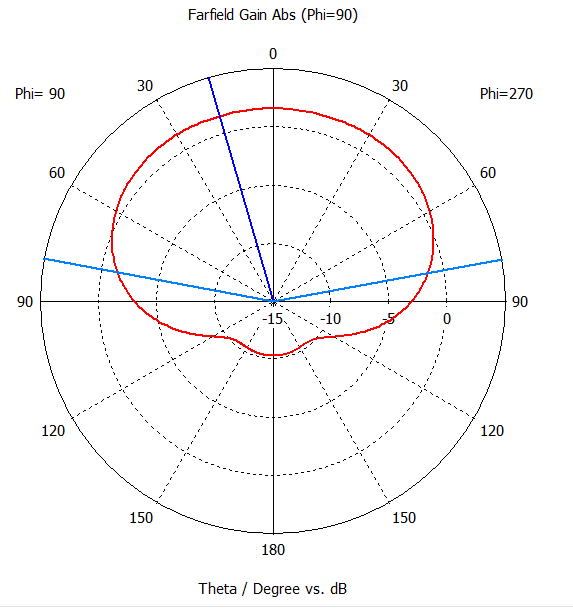
\includegraphics[scale = 0.5]{figures/antennas/qha/qha_6_ff_131}
\caption{Simulated farfield at 131MHz}
\label{fig:QHA_ff_131}
\end{figure}

\begin{figure}[H]
\centering 
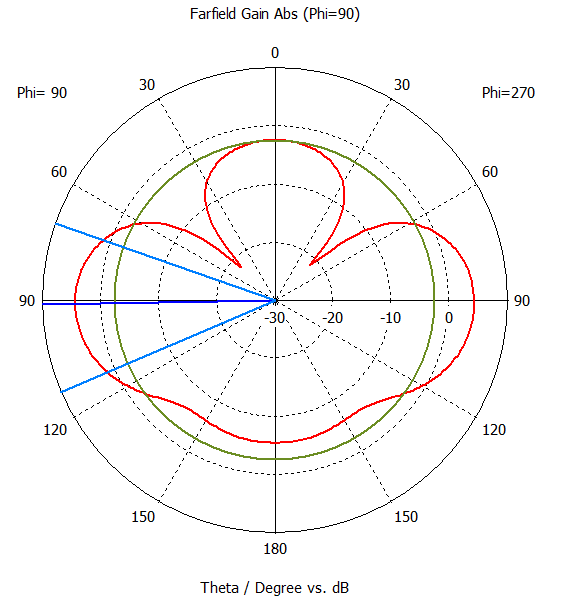
\includegraphics[scale = 0.5]{figures/antennas/qha/qha_6_ff_262}
\caption{Simulated farfield at 262MHz}
\label{fig:QHA_ff_262}
\end{figure}

\begin{figure}[H]
\centering 
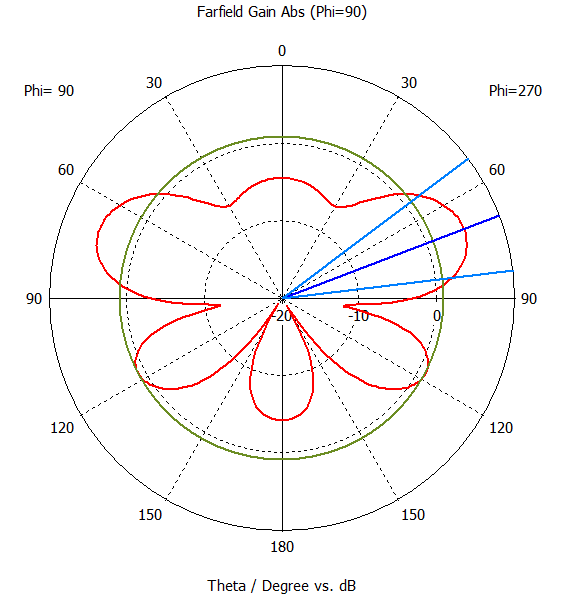
\includegraphics[scale = 0.5]{figures/antennas/qha/qha_6_ff_393}
\caption{Simulated farfield at 393MHz}
\label{fig:QHA_ff_393}
\end{figure}

%%%%%%%%%%%%%%%%%%%%%%%%%%%%%%%%%%%%%%%%%%%%%%%%%%%%%%%%%%%%%%%%%%%%%%%%%%%%%%%%%%%%% Feeding %%%%%%%%%%%%%%%%%%%%%%%%%%%%%%%%%%%%%%%%%%%%%
\subsubsection{Feeding methods}
In figure \ref{fig:QHA2} the feeding of the QHA is done using two discrete ports. When port 1 is fed with a positive phase at $90^\circ$ the QHA will have it's maximum radiation in the forward direction. If the port instead is fed with a negative phase at $90^\circ$ then the QHA will have it's maximum radiation in the backward direction. Other phases will result in non-uniform radiation patterns with one ore more peaks in the azimuth axis. It is easy to believe that it is possible to connect two of the arms of the QHA to a common ground and feed the one port with a phase difference at $90^\circ$ using a $1/4 \lambda $ transmission-line and the other directly from the source depicted in figure \ref{fig:QHA_common}. But this will not work since the geometry of the QHA will change from an electrically perspective. The shortening of the two grounds will affect the flow of the current resulting of only a pattern difference of $45^\circ$ in the farfield which then makes it impossible to archive a omnidirectional radiation pattern and circular polarization. To overcome this is has been shown in \citep{Bai2014} that it is possible to use a feeding network consisting of one second-iteration Moore $180^\circ$ hybrid coupler and two second-iteration Sierpinski $90^\circ$ hybrid couplers. It has also been showen in \citep{Yang2014} that a broadband feed network can be done using an wilkinson powerdivider and broadband $90^\circ$ phase shifters.     

\begin{figure}[H]
\centering 
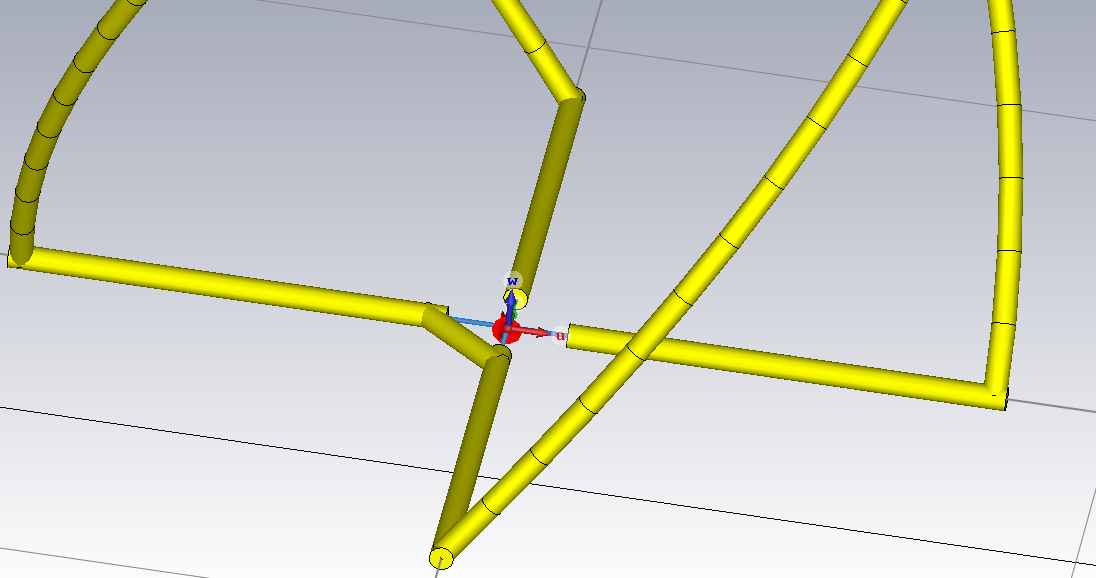
\includegraphics[scale = 0.3]{figures/antennas/qha/qha_6_common_gnd}
\caption{Common GND for the QHA}
\label{fig:QHA_common}
\end{figure}

\subsubsection{Wideband QHA}
As shown previously a QHA in its basic form radiates only at a narrow frequency band. For the S-parameters in figure \ref{fig:QHA_S11} it is seen that at 131MHz the return loss is about -2dB which results in an efficiency at only -5dB. This can be improved using a match network, but the antenna still needs to be a radiating element and therefore the matching can only improve the return-loss and not the bandwidth \citep{Iyver2010}. Therefore some modifications needs to be done at the QHA to improve the bandwith.     

%%%%%%%%%%%%%%%%%%%%%%%%%%%%%%%%%%%%%%%%%%%%%%%%%%%%%%%%%%%%%%%%%%%%%%%%%%%%%%%%%%%%%%%%%%%%%%%%%%%%%%%%%%%%%%%%%%%%%%%%%%%%%%%%%% 


\section{Spiral antennas}


\subsection{Conical Log-Spiral antenna}

\begin{figure}[H]
\centering 
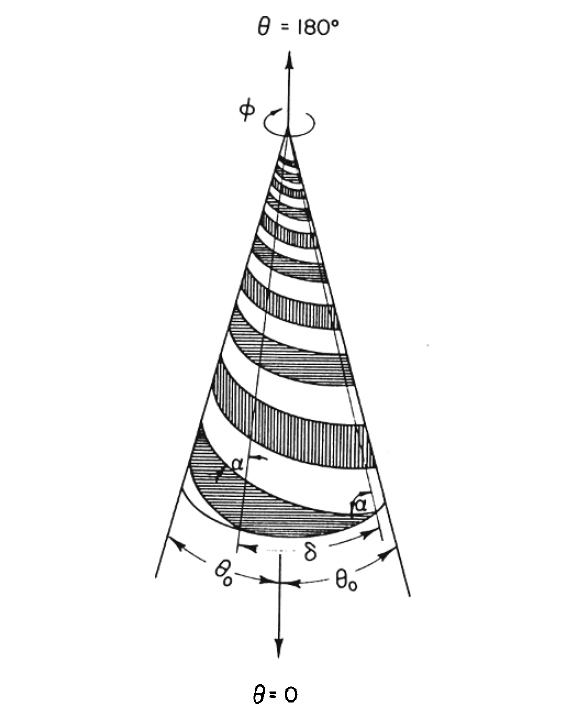
\includegraphics[scale = 0.5]{figures/antennas/spiral/conical_spiral}
\caption{Conical spiral antenna \citep{Rumsey1966}}
\label{fig:con_spi}
\end{figure}


The balanced two arm Conical Log-Spiral Antenna (CLSA) depicted in figure \ref{fig:con_spi} is a derivative of planar spiral antennas which all are frequency independent because the geometry is only described by angles \citep{Balanis2005}. The CLSA consist of two metal strips on the surface of a cone, whose shapes are defined by the equiangular spiral of equation \ref{eq:spiral} \citep{Rumsey1966}.

\begin{equation}
r = e^{\alpha\phi sin(\theta_0)}
\end{equation}
\label{eq:spiral} 

The angle $\alpha$ between the radius and the tangent to the spiral is $cot^{-1}(\alpha)$ and because of the spiral $\theta_0 = 90^\circ$. The CSA do also have circular polarization which makes it usable for satellite communication. 



%%%%%%%%%%%%%%%%%%%%%%%%%%%%%%%%%%%%%%%%%%%%%%%%%%%%%%%%%%%%%%%%%%%%%%%%%%%%%%%%%%%%%%%%%%%%%%%%%%%%%%%%%%%%%%%%%%%%%%%%%%%%%%

\section{Horn antennas}
\section{Printed antennas}










    



   
\chapter{Conclusion}\label{ch:conclusion}
The purpose of this project was to investigate the effects from crosstalk at antenna arrays connected to PAs when they are linearised with DPD. It was shown that it is not necessary to include a mathematical model for the antenna if only one antenna is used at a single amplifier. It was further shown that when introducing two amplifiers with one antenna each the conventional DPD technique was not able to compensate for the crosstalk in the antennas. It was therefore tested to measure the setup as a hole and do DPD with the antennas included into the DPD model. This provided better results with a ACPR about 2dB better. When four amplifiers with one antenna each was introduced the technique still lowers the ACPR with 2dB over all distances between the elements in the antenna array. It was also seen from the AM/AM plots that the DPD model was overcompensating at high power-levels. Therfore the proposed model in figure \ref{fig:dpd_pdpd} is shown to be better than conventional DPD, but that there still are space left to improvements. The measurement in section \ref{ch:ant_meas} of the antennas showed a large variation in the S-parameters due to the spacing of the antenna elements. It was also measured if it had any impact that the amplifiers was biased with same bias voltage but different current due to transistor deviations. It was showed that it had little or no impact on the ACPR when treating the amplifiers with antennas as a hole.     




\bibliography{bib/mybib}
\label{bib:mybiblio}
\appendix
\chapter{Antenna measurements}\label{ch:appAlabel}


\end{document}
